
% * Week 1. (Jul 27) Introduction and R boot camp (Rob & Souhaib)
%   - Lecture 1:  What is Business Analytics? Show case of R.
%   - Lab 1: R exercises
%   - Lecture 2: Introduction to R programming
% - R, Rstudio
% - Rmarkdown
% - Examples:
%     prediction: bulldozers
%     classification: see JWHAT
%     clustering
%   Business analytics vs data science vs statistics vs econometrics 
%   Venn diagrams



\documentclass[14pt, handout]{beamer}
\usepackage{pgf,tikz,pgfpages,amsmath,bm,fancyvrb,animate}
\usepackage{graphicx,bera,booktabs}
\usepackage[australian]{babel}
\usepackage[utf8]{inputenc}
\usepackage{media9}


\definecolor{Orange}{RGB}{255,140,0}
\long\def\TCorange#1{\textcolor{Orange}{#1}}
\long\def\TCblue#1{\textcolor{blue}{#1}}

\newcommand\Wider[2][3em]{%
\makebox[\linewidth][c]{%
  \begin{minipage}{\dimexpr\textwidth+#1\relax}
  \raggedright#2
  \end{minipage}%
  }%
}

\usetheme{Monash}
\def\biz{\begin{itemize}[<+-| alert@+>]}
\def\eiz{\end{itemize}}
\def\ben{\begin{enumerate}[<+-| alert@+>]}
\def\een{\end{enumerate}}

%\AtBeginSubsection[]  
%  {  
%    \begin{frame}<*>{Outline}  
%      \tableofcontents[currentsection,currentsubsection]  
%    \end{frame}  
%  }


\graphicspath{{../figures/}}

\title[Introduction to Business Analytics and R]{Business Analytics}
\author{Week 1.\\ Introduction to Business Analytics \& R}
\date{29 July 2015}

\DefineShortVerb{\"}
\def\FancyVerbFormatCom{\color[rgb]{0.6,0,1}\relax}


\def\source#1{\vspace{-0.4cm}\par{\fontsize{6}{8}\sffamily \url{#1}}}
\def\inlinesource#1{\hbox{\fontsize{6}{8}\sffamily \url{#1}}}

 
\begin{document}

\begin{frame}[plain]{}
\maketitle
\begin{textblock}{11}(0.5,1.3){\color{white}\large
\textbf{ETC3250}}
\end{textblock}

\end{frame}


\begin{frame}{Example 1: Prediction}\fontsize{13}{14}\sf

\begin{block}{Kaggle competition: bulldozer auction prices}
\textbf{Problem}: Predict a bulldozer sale price based on known characteristics:
\begin{itemize}
\item Year made
\item Sale date
\item Machine hours
\item Product group
\item Type of enclosure
\end{itemize}
\end{block}
\pause
\begin{enumerate}
\item How could you improve the model?
\item How to use model to predict bulldozer prices when some information missing?
\item Does predicting log price make sense?
\end{enumerate}


\end{frame}
\begin{frame}{Example 2: Classification}

\begin{block}{Identification of high gold potentials}
\textbf{Problem}: Identify high gold potentials at deep layers from soil properties measurements at multiple locations. 
\end{block}

\centerline{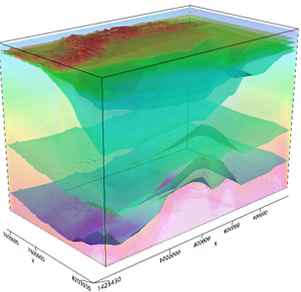
\includegraphics[scale=0.4]{../figures/layers.png}}

\end{frame}

\begin{frame}[fragile]\frametitle{Example 2: Classification}
	
{\scriptsize
\begin{verbatim}
Longitude Latitude   Ag   As   Ce   Co    Sr Ta Tb Te  Th    Mo   Au
   43.1723  22.3255 5.00  2.0 3.67 1.39  0.46  1  4  1 5.5   8.8  2.35
   43.1732  22.3255 0.63 15.5 1.33 3.94 12.95  1  1  2 1.5 160.0  4.29
   43.1742  22.3255 3.81  2.5 0.67 1.44  2.73  1  1  1 0.5   2.0  21.94
\end{verbatim}
}

ADD Gold/No gold \\
ADD Low, Medium and High gold

\begin{enumerate}
\item How to apply multi-class classification with binary classifiers?
\item Can you give an example of unbalanced classification problem?
\item Does predicting log price make sense?
\end{enumerate}

\end{frame}

\end{document}